\section{Inspiration from the Primate Visual Cortex}
\label{sec:pvc}
\todo[inline,author=Mikael]{auhhhej}

\begin{figure}[h!]
\centering
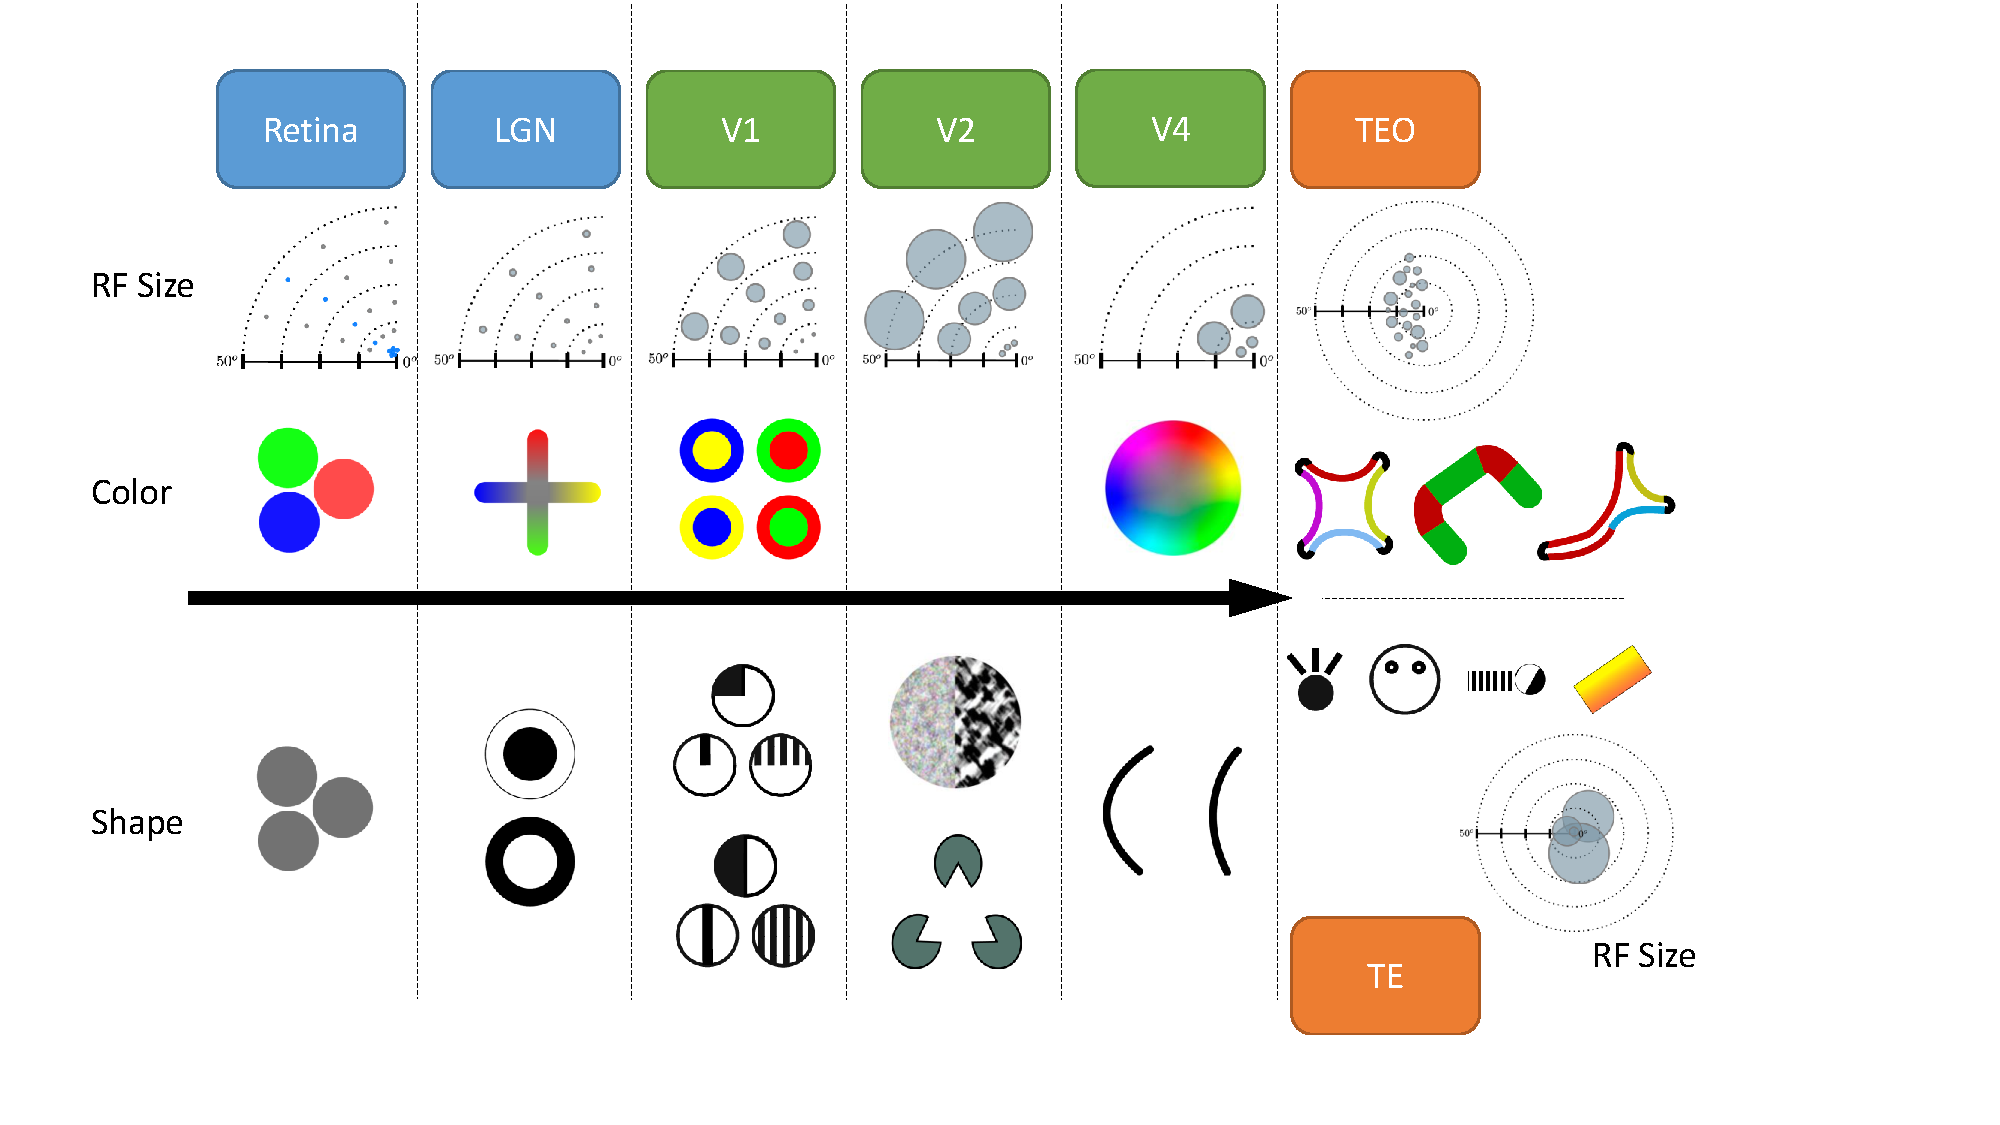
\includegraphics[width=1.0\textwidth]{graphics/pvc_figure1}
\caption[Object Recognition Pathway]{
Simplified sketch of the hierarichal structure of the object recognition pathway in the primate visual system.
The vertical lines separate layers from the low layers on the left, to the higher, more complex layers, on the right.
Up until layers TEO and TE, the compositions can be split into two categories: color and shape.
Also illustrated are the Receptive Field sizes (RF Size) of the individual layers.
Adapted from \cite{kruger2013deep}.
}
\label{fig:pcv1}
\end{figure}